% GHOST system model with the real intermediate tensors of one request
% (ResNet-20, split after block 3, rho = 10, CIFAR-10 test image 1398), produced by ghost2/fig_tensors.py.
% Drawn at IEEE \textwidth (7.16in) so fonts render at true size.
\documentclass[tikz,border=1pt,10pt]{standalone}
\usepackage[T1]{fontenc}
\usepackage{mathptmx}
\usepackage{courier}
\usepackage{graphicx}
\usetikzlibrary{arrows.meta,calc,shapes.geometric}
\definecolor{navy}{HTML}{011E4B}
\definecolor{gold}{HTML}{FAB001}
\definecolor{sky}{HTML}{87C6E9}
\definecolor{alert}{HTML}{EE1C23}
\def\TokHex{e1817c66}
\def\CtHex{d06c51cc}
\def\PredClass{Horse}
\def\ProbList{0.056,0.000,0.013,0.041,0.001,0.066,0.000,0.813,0.008,0.002}
\def\WRows{16}\def\WtRows{20}

\graphicspath{{arch_assets/}}
\tikzset{
  >={Stealth[length=2.2mm,width=1.7mm]},
  font=\footnotesize,
  zone/.style={draw=#1,line width=1.1pt,rounded corners=3pt},
  head/.style={fill=#1,text=white,font=\footnotesize\bfseries,anchor=north west,
               inner xsep=4pt,inner ysep=2.5pt,rounded corners=1.5pt},
  ttl/.style={text=navy,align=center,inner sep=1pt,font=\footnotesize},
  f/.style={->,draw=navy,line width=0.9pt},
  fo/.style={->,draw=navy,line width=0.9pt,dash pattern=on 3pt off 2pt},
  n/.style={circle,fill=navy,text=white,font=\scriptsize\bfseries,inner sep=0pt,minimum size=4mm},
  lab/.style={font=\scriptsize,text=navy,inner sep=1pt},
}
% feature-map stack: four channels, front tile 1cm, centred at (#1,#2), files #3{0..3}
\newcommand{\fstack}[3]{%
  \foreach \k in {3,2,1,0}{%
    \node[inner sep=0pt,anchor=south west,draw=navy,line width=0.4pt]
      at ({#1-0.695+\k*0.13},{#2-0.695+\k*0.13}) {\includegraphics[width=1cm]{#3\k}};}}
\newcommand{\tile}[4]{% single image tile #3 of width #4 centred at (#1,#2)
  \node[inner sep=0pt,draw=navy,line width=0.5pt] at (#1,#2) {\includegraphics[width=#4]{#3}};}
\newcommand{\padlock}[2]{%
  \begin{scope}[shift={(#1,#2)}]
   \draw[navy,line width=1.3pt] (-0.11,0.1) -- (-0.11,0.2) arc (180:0:0.11) -- (0.11,0.1);
   \fill[navy,rounded corners=1pt] (-0.19,-0.17) rectangle (0.19,0.12);
   \fill[gold] (0,-0.02) circle (0.045);
  \end{scope}}
\newcommand{\cuboid}[4]{% x, y(centre), width, height
  \fill[sky,draw=navy,line width=0.5pt] (#1,#2-#4/2) rectangle ++(#3,#4);
  \fill[navy,draw=navy,line width=0.5pt] (#1,#2+#4/2) -- ++(0.12,0.12) -- ++(#3,0) -- ++(-0.12,-0.12) -- cycle;
  \fill[gold,draw=navy,line width=0.5pt] (#1+#3,#2-#4/2) -- ++(0.12,0.12) -- ++(0,#4) -- ++(-0.12,-0.12) -- cycle;}
\begin{document}
\begin{tikzpicture}
% =============================================================== zones
\draw[zone=navy] (0,0) rectangle (2.75,10);
\node[head=navy] at (0.08,9.92) {Client};
\draw[zone=navy] (3.05,0) rectangle (15.0,10);
\node[head=navy] at (3.13,9.92) {Edge Device};
\draw[zone=gold] (3.25,4.95) rectangle (14.65,9.35);
\node[head=gold,text=navy] at (3.33,9.27) {Trusted Execution Environment (TEE)};
\draw[zone=alert,dash pattern=on 4pt off 2pt] (3.25,0.2) rectangle (14.65,4.6);
\node[head=alert] at (3.33,4.52) {Rich Execution Environment (REE)};
\node[head=alert,anchor=south east] at (14.57,0.28) {Adversary Controlled};
\draw[zone=navy] (15.3,0) rectangle (18.3,10);
\node[head=navy] at (15.38,9.92) {Model Owner Cloud};

% =============================================================== client
\tile{1.375}{7.2}{input}{1.4cm}
\node[ttl,anchor=south] at (1.375,8.0) {Input Image};
\node[draw=navy,fill=white,rounded corners=2pt,line width=0.6pt,font=\footnotesize\ttfamily\bfseries,text=navy,inner sep=2.5pt] (tok) at (1.375,5.95) {\TokHex};
\node[ttl,anchor=north] at (1.375,5.6) {Access Token};
\draw[navy,line width=0.6pt] (1.375,6.5) -- (tok.north);
% prediction bars
\node[ttl,anchor=south] at (1.375,3.3) {Prediction};
\foreach \c [count=\i from 0] in {plane,car,bird,cat,deer,dog,frog,horse,ship,truck}{%
  \pgfmathsetmacro{\p}{{\ProbList}[\i]}
  \pgfmathsetmacro{\yy}{3.0-\i*0.245}
  \node[lab,anchor=east,font=\scriptsize] at (0.95,\yy) {\c};
  \ifnum\i=7
    \fill[gold,draw=navy,line width=0.4pt] (1.0,\yy-0.09) rectangle ++({1.25*\p},0.18);
    \node[lab,anchor=west,font=\scriptsize\bfseries] at ({1.0+1.25*\p},\yy) {\pgfmathprintnumber[fixed,precision=2]{\p}};
  \else
    \fill[sky,draw=navy,line width=0.4pt] (1.0,\yy-0.09) rectangle ++({max(1.25*\p,0.02)},0.18);
  \fi}
\draw[navy,line width=0.6pt] (1.0,3.15) -- (1.0,0.7);

% =============================================================== TEE
% token and budget check: shield + budget gauge
\begin{scope}[shift={(4.2,7.35)}]
  \fill[navy] (0,0.55) .. controls (0.25,0.45) .. (0.42,0.45) -- (0.42,0.05) .. controls (0.42,-0.3) .. (0,-0.5)
              .. controls (-0.42,-0.3) .. (-0.42,0.05) -- (-0.42,0.45) .. controls (-0.25,0.45) .. cycle;
  \draw[gold,line width=1.6pt,line cap=round,line join=round] (-0.2,0.0) -- (-0.04,-0.17) -- (0.22,0.2);
  \foreach \j in {0,...,7}{\ifnum\j<3 \fill[navy] \else \draw[navy,line width=0.5pt,fill=white] \fi
     ({-0.62+\j*0.16},-0.82) rectangle ++(0.12,0.2);}
\end{scope}
\node[ttl,anchor=south] at (4.2,8.0) {Token and\\ Budget Check};
\fstack{6.3}{7.2}{a}
\node[ttl,anchor=south] at (6.3,8.0) {First\\ Convolution};
\fstack{8.45}{7.2}{R}
\node[ttl,anchor=south] at (8.45,8.0) {Mixing and\\ One-Time Masking};
\fstack{11.25}{7.2}{y}
\node[ttl,anchor=south] at (11.25,8.0) {Unmasking\\ and Unmixing};
\tile{13.6}{7.2}{ct}{1.0cm}
\padlock{13.95}{7.6}
\node[ttl,anchor=south] at (13.6,8.0) {Feature\\ Encryption};
% key store
\node[inner sep=1.5pt,draw=gold,line width=1.1pt,rounded corners=1.5pt,fill=white] (keys) at (13.55,5.65)
  {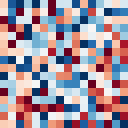
\includegraphics[width=0.55cm]{B}\hspace{2pt}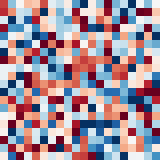
\includegraphics[width=0.55cm]{A}};
\node[ttl,anchor=east] at (keys.west) {Key Store};

% =============================================================== REE
\fstack{8.45}{3.25}{xt}
\node[ttl,anchor=north] at (8.45,2.45) {Masked\\ Activation};
\begin{scope}[shift={(9.85,3.25)}]
  \foreach \j in {-0.27,-0.09,0.09,0.27}{
    \draw[navy,line width=0.7pt] (\j,0.4) -- (\j,0.52); \draw[navy,line width=0.7pt] (\j,-0.4) -- (\j,-0.52);
    \draw[navy,line width=0.7pt] (0.4,\j) -- (0.52,\j); \draw[navy,line width=0.7pt] (-0.4,\j) -- (-0.52,\j);}
  \fill[navy,rounded corners=1.5pt] (-0.4,-0.4) rectangle (0.4,0.4);
  \fill[gold] (-0.2,-0.2) rectangle (0.2,0.2);
\end{scope}
\node[ttl,anchor=south] at (9.85,3.85) {Accelerator\\ Convolution};
\fstack{11.25}{3.25}{yt}
\node[ttl,anchor=north] at (11.25,2.45) {Masked\\ Output};
\tile{6.3}{3.25}{Wt}{1.15cm}
\node[ttl,anchor=east] at (5.6,3.25) {Obfuscated\\ Weights};

% =============================================================== cloud
\node[ttl,anchor=south] at (16.8,8.0) {Suffix Network};
\fstack{16.25}{7.2}{f}
\cuboid{17.1}{7.2}{0.22}{0.9}
\cuboid{17.48}{7.2}{0.2}{0.65}
\cuboid{17.83}{7.2}{0.16}{0.4}
\foreach \t/\yy/\s in {Probability Vector/5.0/1,Top-1 Confidence/4.6/0,Label Only/4.2/0}{
  \ifnum\s=1 \node[fill=navy,text=white,rounded corners=2.2mm,font=\scriptsize\bfseries,minimum width=2.45cm,inner ysep=2pt] at (16.8,\yy) {\t};
  \else \node[draw=navy,fill=white,text=navy,rounded corners=2.2mm,font=\scriptsize,line width=0.6pt,minimum width=2.45cm,inner ysep=2pt] at (16.8,\yy) {\t}; \fi}
\node[ttl,anchor=north] at (16.8,3.9) {Output Release\\ Policy};
\tile{16.8}{1.25}{W}{1.15cm}
\node[ttl,anchor=south] at (16.8,1.85) {Attestation and\\ Provisioning};

% =============================================================== legend
\draw[f] (3.5,0.5) -- ++(0.6,0) node[right,lab]{Online inference};
\draw[fo] (5.95,0.5) -- ++(0.6,0) node[right,lab]{One-time setup};

% =============================================================== one-time setup
\draw[fo] (16.2,1.0) -- (5.95,1.0) -- (5.95,2.65);
\draw[fo] (16.2,1.6) -- (14.83,1.6) |- (keys.east);

% =============================================================== online inference
\draw[f] (2.075,7.2) -- node[n,above=2pt]{1} (3.65,7.2);
\draw[f] (4.75,7.2) -- node[n,above=2pt]{2} (5.6,7.2);
\draw[f] (7.0,7.2) -- (7.75,7.2);
\draw[f] (8.45,6.5) -- node[n,left=2pt]{3} (8.45,3.95);
\draw[f] (9.15,3.25) -- (9.3,3.25);
\draw[f] (10.4,3.25) -- (10.55,3.25);
\draw[f] (6.65,2.65) -- (6.65,1.5) -| (9.85,2.65);
\draw[f] (11.25,3.95) -- node[n,right=2pt]{4} (11.25,6.5);
\draw[f] (10.55,7.2) -- node[n,above=2pt]{5} (9.15,7.2);
\draw[f] (11.95,7.2) -- node[n,above=2pt]{6} (13.1,7.2);
\draw[f] (14.1,7.2) -- node[n,above=2pt]{7} (15.55,7.2);
\draw[f] (16.8,6.5) -- (16.8,5.22);
\draw[f] (18.03,4.6) -- (18.1,4.6) -- (18.1,-0.4) -| node[pos=0.25,n,below=2pt]{8} (1.375,0.65);
\end{tikzpicture}
\end{document}
